\documentclass[hyperref={pdfpagelabels=false},xcolor=dvipsnames,12pt,aspectratio=169]{beamer}
\let\Tiny=\tiny

\usepackage[czech]{babel}
\usepackage{xltxtra}
\usepackage{hyperref}
\hypersetup{colorlinks=false,hidelinks}
\setromanfont{DejaVu Serif}
\setsansfont{DejaVu Sans}
\setmonofont{DejaVu Sans Mono}


\setbeamertemplate{navigation symbols}{}

\mode<presentation>
{
  %\usetheme{Frankfurt}
  %\usecolortheme{wolverine}
  %\usetheme[height=7mm]{Rochester}
  \usetheme{Madrid}
  \usecolortheme[RGB={18,90,158}]{structure}
}

\title{Kostra přednášky}
\author{Ondřej Caletka}
\institute[CESNET, z. s. p. o.]{\includegraphics[width=6cm]{fig/cesnet-20let-rozsirena}}
\logo{\includegraphics[width=2cm]{fig/cesnet-20let-zakladni}}
%\date{5.~listopadu~2013}


\begin{document}

\section*{Úvod}

{
\setbeamertemplate{logo}{}
\begin{frame}
 \titlepage
 \begin{figure}
		\includegraphics[width=2ex]{fig/cc}
		\hspace*{0.5ex}
		\includegraphics[width=2ex]{fig/by}

		\tiny Uvedené dílo podléhá licenci Creative Commons Uveďte autora 3.0 Česko.
 \end{figure}
\end{frame}
\begin{frame}
 \frametitle{O~sdružení CESNET}
 \begin{figure}
     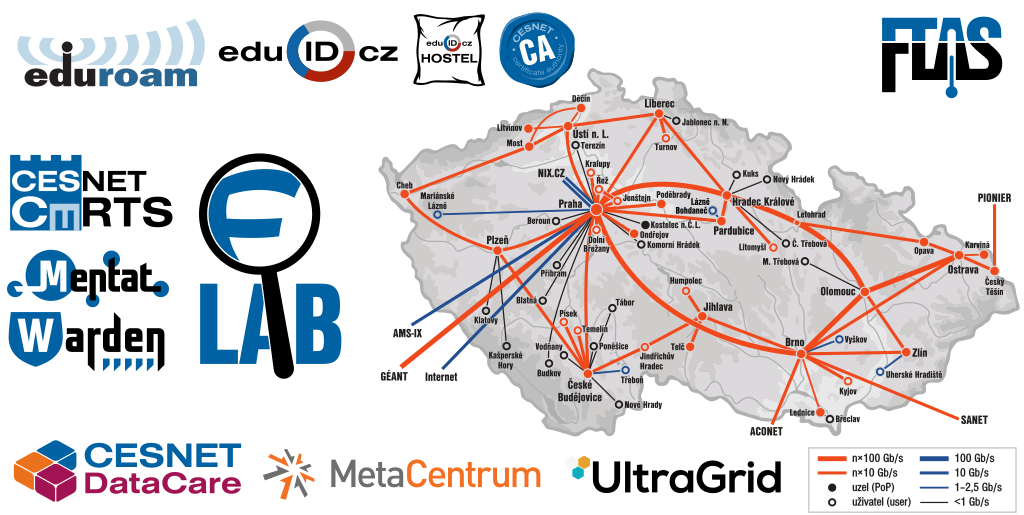
\includegraphics[width=0.9\textwidth]{fig/osdruzeni169}
 \end{figure}
\end{frame}
}

\begin{frame}
 \frametitle{Obsah}
 \tableofcontents
\end{frame}

\section{První okruh}

\begin{frame}
	\frametitle{První slide}
	\begin{block}{Titulek bloku}
		\begin{itemize}
			\item odrážka v~bloku
			\item odrážka v~bloku
			\item odrážka v~bloku
		\end{itemize}
	\end{block}
	\begin{alertblock}{Důležitý blok}
		\begin{itemize}
			\item odrážka v~bloku
			\item odrážka v~bloku
			\item odrážka v~bloku
		\end{itemize}
	\end{alertblock}
\end{frame}

\begin{frame}
	\frametitle{Slide s~odrážkami}
	\begin{itemize}
		\item 
		\item 
		\item 
		\item 
		\item 
		\item 
		\item 
	\end{itemize}
\end{frame}

\begin{frame}[fragile]
	\frametitle{Slide s~verbatimem}
	\begin{itemize}
		\item musí být fragile
		\item krátké citate takto
		\begin{itemize}
				\item \verb|01:00:5e| 
				\item \verb|33:33|
		\end{itemize}
		\item dlouhé do prostředí verbatim
		\begin{verbatim}
Lorem ipsum amit bla bla 
      bla
		\end{verbatim}
	\end{itemize}
\end{frame}

\section*{Závěr}
{
\setbeamertemplate{logo}{}
\begin{frame}
 \begin{center}
 \large Děkuji za pozornost

 \vspace{1cm}
 Ondřej Caletka

 \texttt{Ondrej.Caletka@cesnet.cz} \\
 \texttt{\href{https://xn--ondej-kcb.caletka.cz}{https://Ondřej.Caletka.cz}}
 \begin{figure}
 \includegraphics[width=8cm]{fig/cesnet-20let-rozsirena}
 \end{figure}
 \end{center}
\end{frame}
}
\end{document}
